%% LaTeX2e class for seminar theses
%% sections/content.tex
%% 
%% Karlsruhe Institute of Technology
%% Institute for Program Structures and Data Organization
%% Chair for Software Design and Quality (SDQ)
%%
%% Dr.-Ing. Erik Burger
%% burger@kit.edu
%%
%% Version 1.0.2, 2020-05-07

\section{Technische  Funktionsweise der C2C-Kommunikation}
\label{ch:FirstContentSection}

Im folgenden Abschnitt wird die Funktionsweise der C2C-Kommunikation und die dafür benötigte Infrastruktur näher beschrieben. Zuerst wird in Kapitel \ref{sec:FirstContentSection:ZeroSubSection} der Standard WAVE vorgestellt, der die moderne C-ITS Kommunikation definiert, und deren Bausteine werden näher beschrieben. Das Ziel von diesem Standard ist es, eine einheitliche Schnittstelle für die Car-to-Car und Car-to-Infrastructure, bzw. Nahbereichskommunikation zu ermöglichen.

Im Abschnitt \ref{sec:FirstContentSection:FirstSubSection} wird die Public-Key Infrastruktur (PKI) beschreiben, die für den sicheren Nachrichtenaustausch zwischen den Verkehrsteilnehmern essenziell ist. Es wird auf die kryptografischen Prozesse und auf die organisatorische Stellenhierarchie eingegangen, die für die Implementierung einer PKI nötig sind. Abschließend werden einige Besonderheiten der europäischen PKI erwähnt.

Im Abschnitt \ref{sec:FirstContentSection:SecondSubSection} wird auf die Nachrichtenformate der C2C-Kommunikation eingegangen, sowie auf die darin gespeicherten Daten, die möglicherweise zur Identifikation des Fahrzeugs benutzt werden können. Dieses technische Thema bildet eine Grundlage für Herstellbarkeit des Personenbezugs aus den Fahrdaten, deren Möglichkeit in weiteren Kapiteln analysiert wird.

\subsection{Standard for Wireless Access in Vehicular Environments (WAVE)}
\label{sec:FirstContentSection:ZeroSubSection}

Wie vorhin erwähnt, besteht eine C-ITS nicht nur aus Fahrzeugen, die miteinander kommunizieren, sondern auch verschiedenen anderen Infrastrukturkomponenten (z.B. Ampelanlagen und intelligente Verkehrsschilder). Da sowohl Fahrzeuge als auch Infrastrukturkomponenten von verschiedenen Herstellern produziert werden, wird ein gemeinsamer Standard benötigt, um reibungslose Kommunikation und Datenaustausch zu gewährleisten. Daher hat das IEEE Konsortium eine Reihe von Standards geschaffen, die gemeinsam \emph{IEEE 1609 Family of Standards for Wireless Access in Vehicular Environments (WAVE)} genannt werden \cite{WAVE}. WAVE beschreibt die Architektur, Kommunikationsmodelle, Verwaltungsstrukturen und Sicherheitsmechanismen im Kontext von C-ITS. Der vorher erwähnte WLAN-Funkstandard IEEE 802.11p ist ebenfalls ein Baustein von WAVE und wird hier als ein einheitlicher Standard für Nahbereichskommunikation verwendet. 

Die zwei Hauptkomponenten der WAVE Architektur sind \emph{On Board Unit (OBU)} - ein direkt im Fahrzeug installiertes Computer- und Sendegerät, und am Straßenrand installiertes \emph{Road Side Unit (RSU)} - siehe Abbildung \ref{fig:vanet}. Die OBUs tauschen Nachrichten mit anderen Fahrzeugen in der Nähe durch einen direkten Kanal aus, und falls das Zielfahrzeug zu weit weg ist aber sich trotzdem im gleichen Netz befindet, kommunizieren sie durch mehrere Hops \cite{VANET}. Die Fahrzeuge können sich durch RSUs am Straßenrand mit dem Internet verbinden.

\begin{figure}
	\centering
	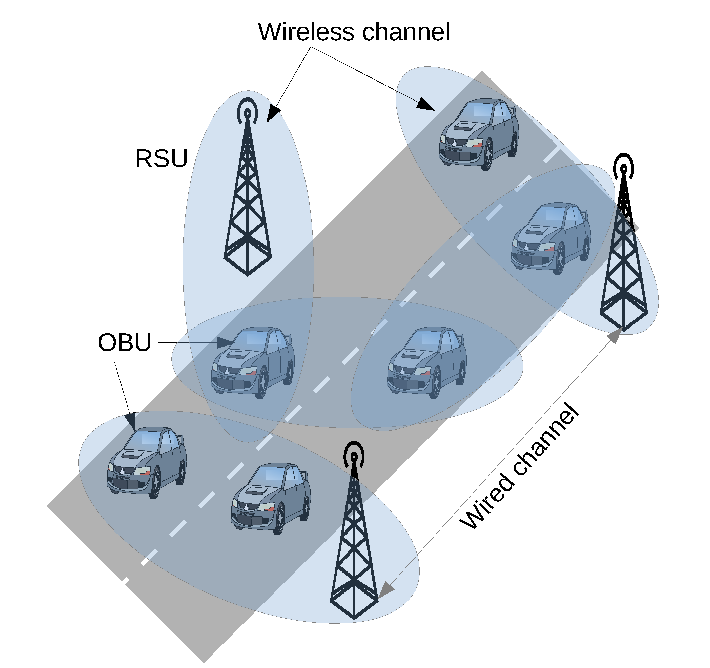
\includegraphics[width=0.7\linewidth]{images/VANET}
	\caption{Überblick über die WAVE Architektur \cite{VANET}}
	\label{fig:vanet}
\end{figure}


\subsection{Public-Key Infrastruktur}
\label{sec:FirstContentSection:FirstSubSection}

Der oben beschriebene Nachrichtenaustausch zwischen Fahrzeugen beruht auf Public-Key Kryptografie, somit werden die Nachrichten mit einer Signatur und einem Zertifikat versehen, die von einer zentralen Stelle ausgegeben werden. Eine kryptographische Signatur ist (analog zu einer Unterschrift) eine Bestätigung, dass die Nachricht tatsächlich von dem Versender stammt und nicht auf dem Weg verändert wurde. Der Empfänger kann dies überprüfen, in dem er die zentrale Stelle kontaktiert und eine Authentizität-Anfrage macht. Die Integrität der Nachricht kann er direkt durch die Signatur verifizieren. Allerdings werden die Nachrichten selbst nicht verschlüsselt und können von allen Verkehrsteilnehmern gelesen werden. Das heißt, dass alle darin enthaltenen Daten ebenfalls von jedem mitgelesen können, was zu datenschutzrechtlichen Problemen führen könnte. 
 
Um den Nachrichtenaustausch zu ermöglichen, braucht man eine entsprechende Public-Key Infrastruktur (PKI), die aus einer oder mehreren Certification Authorities (CAs) besteht. Eine CA ist eine zentrale Stelle die in der Lage ist, digitale Zertifikate zu produzieren, diese Zertifikate den End-Entitäten zu erteilen und später ihre Authentizität zu verifizieren. Als End-Entitäten versteht man ITS-Stationen (u.a. Fahrzeuge), die die erstellten Zertifikate für die Kommunikation untereinander verwenden. Es gibt zwei Arten von Zertifikaten: ein langlebiges Enrolment Credential (EC) und ein kurzzeitgültiges Authorization Ticket (AT). Die Pseudonymität des Datenaustauschs wird durch ständigen Wechsel des ATs gewährleistet, womit die Nachricht signiert wird. Der Enrolment Credential wird hingegen nicht mit der Nachricht übertragen und ist nur den PKI Komponenten bekannt \cite{Strubbe2017}. 

Die PKI wird aus drei Stufen zusammengesetzt \cite{SecurityCITS}: 
\begin{itemize}
	\item Root-CAs (erstellen Zertifikate für untergeordnete CAs)
	\item Mindestens zwei Sub-CAs
	\item End-Entitäten (EEs)
\end{itemize}

Darüber hinaus gibt es zwei Arten von Sub-CAs: Enrolment Authorities (EA) und Authorization Authorities (AA). Die EAs erstellen langlebige Zertifikate für End-Entitäten, die für die Authentifizierung innerhalb der PKI verwendet werden - Enrolment Credentials (ECs). Die AAs hingegen stellen kurzzeitige Zertifikate zur Verfügung, mit denen die End-Entitäten (z.B. Fahrzeuge) untereinander kommunizieren können ohne die Pseudonymität von einzelnen Entitäten zu verletzen - Authorization Tickets (ATs). Der schematische Aufbau von einer PKI wird in der Abbildung \ref{fig:pki} verdeutlicht.

\begin{figure}
	\centering
	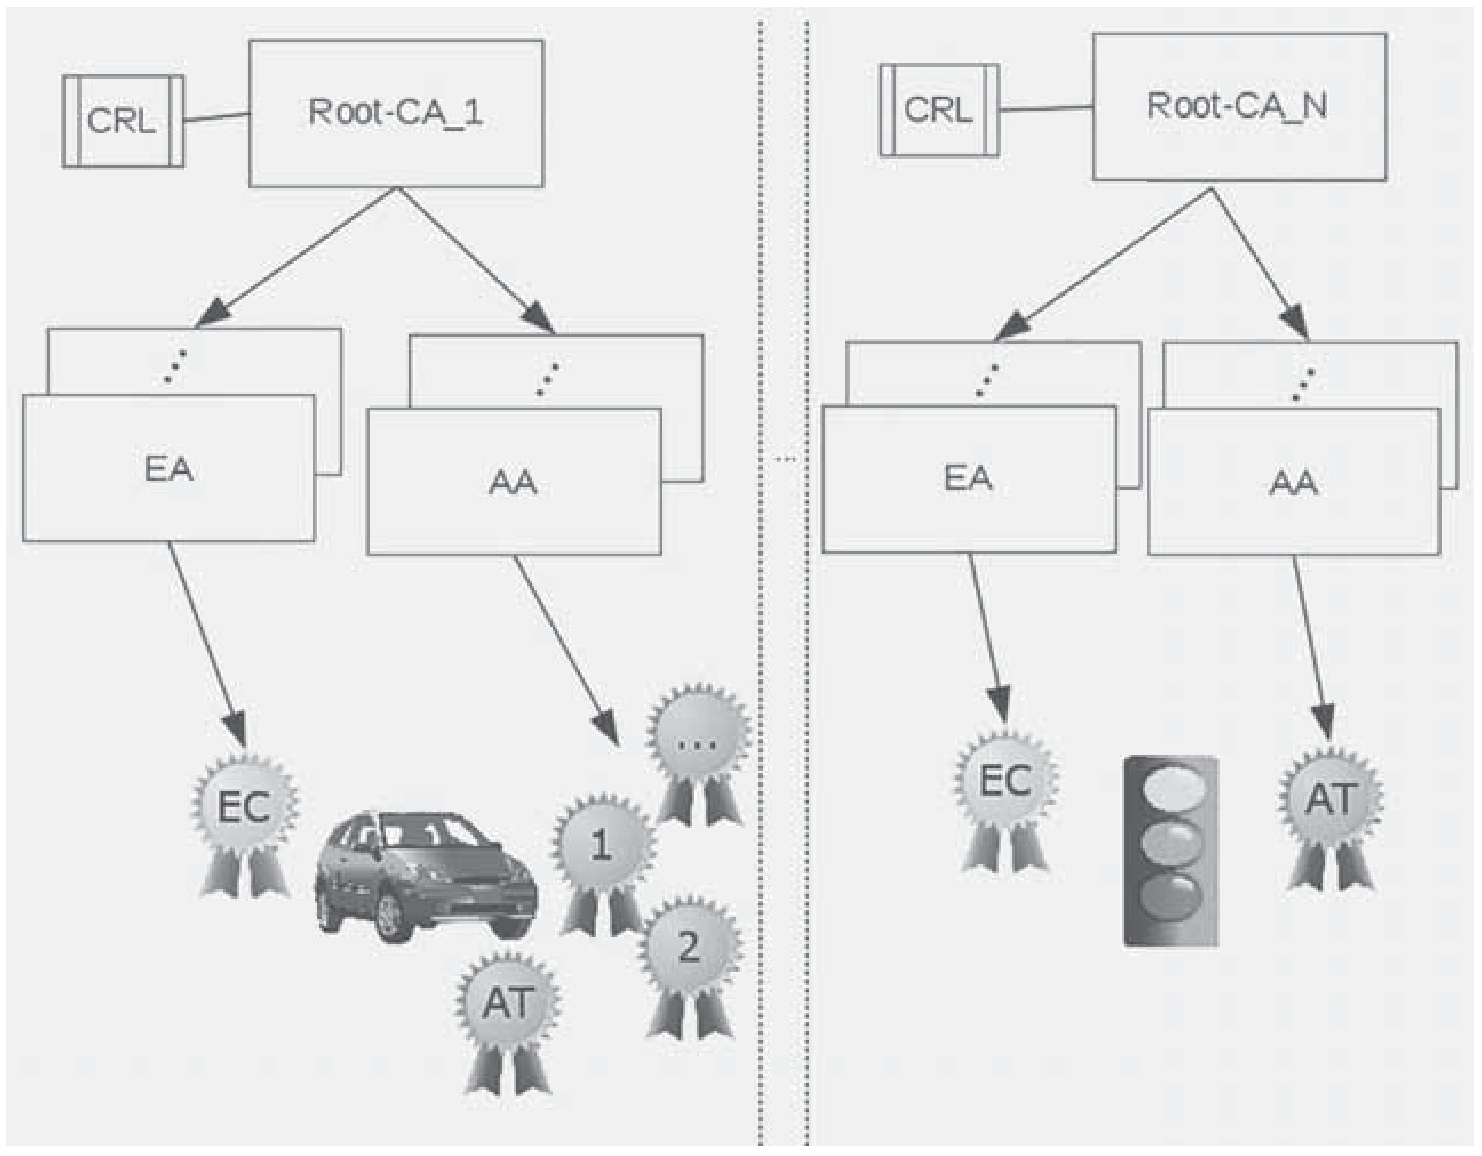
\includegraphics[width=0.7\linewidth]{images/PKI}
	\caption[Aufbau einer PKI für C2X Kommunikation]{Aufbau einer PKI für C2X Kommunikation \footnotemark}
	\label{fig:pki}
\end{figure}
\footnotetext{\emph{Strubbe}, In: DuD 2017, 223}

Bevor jegliche Kommunikation stattgefunden hat, muss sich die End-Entität (EE) zunächst bei der zugehörigen Enrolement Authority (EA) registrieren und ein Enrolment Credential (EC) erhalten, das mehrere Jahre gültig ist. Die EA bekommt dabei die Registrierungsinformationen von der EE, zum Beispiel ihre Fahrzeugidentifizierungsnummer und ihren öffentlichen Schlüssel. Diese Information wird verschlüsselt übermittelt und ist nicht öffentlich verfügbar. Die EE signiert den initialen Zertifikatsrequest mit ihrem eingebauten privaten Schlüssel und übermittelt ihn an die EA. Falls die Daten übereinstimmen, erhält die EE einen Enrolment Credential.

Mit einem validen EC kann die EE weiterhin kurzzeitgültige Authorization Tickets (AT) bei der Authorization Authority (AA) beantragen. ATs sind wie vorhin beschrieben kurzzeitgültige Zertifikate für C2X Kommunikation, die oft gewechselt werden und somit der Senderpseudonymität dienen. Die Nachrichten sollten keinen eindeutigen Identifikator erhalten, damit kein Personenbezug hergestellt werden kann. Daher werden sie mit ATs signiert und nicht mit den langlebigen ECs, die für ein Fahrzeug über mehrere Jahre gültig ist. 

Ein AT wird von einer Entität bei der AA beantragt. Die Anfrage an die AA enthält unter anderem verschlüsselte Daten, die nur von der entsprechenden Enrolment Authority (EA) ausgelesen werden können \cite{ETSI2018}, darunter das langlebige EC von der Entität. Eine AA kann diese Daten nicht auslesen, da sie verschlüsselt sind, also leitet sie diesen Teil der Anfrage an die zugehörige EA. Die EA entschlüsselt die Daten, bestätigt die Authentizität der End-Entität mit dem angehängten EC und schickt eine Statusmeldung an die AA, ohne diese zusätzliche Information preiszugeben. Es ist wichtig, die EA und AA organisatorisch getrennt zu halten, da sonst bei der AT-Anfrage eine Zuordnung zu der End-Entität bzw. ihrem EC möglich wäre.

Nachdem die mit dem AT signierte Nachricht erfolgreich an die empfangende EE übermittelt wurde, nutzt sie den AT um die Nachricht zu verifizieren. Dies erfolgt mittels einer Kettenprüfung durch die AA und die entsprechende Root-CA, wodurch die Authentizität der Nachricht festgestellt wird.

In Europa ist zusätzlich zu der oben beschriebenen PKI eine globale Vertrauensliste vorgesehen, die innerhalb der europäischen Grenzen alle vertrauenswürdige Root-CA-Zertifikate beinhaltet. Diese wird von einem zentralen Trust List Manager erstellt und elektronisch signiert. Somit wird die Interoperabilität von europäischen PKIs über Grenzen sichergestellt, was durch die IVS-RL vorgeschrieben wird\footnote{\emph{Jochum}, In: ZD 2020, 497}. Darüber hinaus ist es wichtig, die nicht mehr vertrauenswürdigen Zertifikate zurückziehen zu können - dies wird durch sogenannte Certificate Revocation Lists sichergestellt. Diese werden allen PKI-Teilnehmern von der jeweiligen Root-CA zur Verfügung gestellt und enthalten die Liste mit allen revozierten Zertifikaten.  

\subsection{Nachrichtenformate}
\label{sec:FirstContentSection:SecondSubSection}

Die Nachrichtenformate, die für die oben beschriebene PKI nötig sind, wurden von dem Europäischen Institut für Telekommunikationsnormen (ETSI) definiert. Im Weiteren wird auf \cite{ETSI2018} verwiesen, in dem die Paketstruktur für gesicherte C2X-Nachrichten und deren Zertifikatsformat festgelegt wurde. 

Der grobe Aufbau einer gesicherten C2X-Nachricht wird in der Abbildung \ref{fig:nachrichtenaufbau} dargestellt. Sie enthält unter anderem die ECDSA-Signatur (\cite{Barker2013}), den Verifikationsschlüssel des Senders und die eigentliche Nachricht, die im Payload gespeichert ist. Für die Car-2-Car Kommunikation sind zurzeit zwei Nachrichtenformate vorgesehen:
\begin{itemize}
	\item die Cooperative Awareness Message (CAM) und die 
	\item Decentralized Environmental Notification Message (DENM) \cite{ETSI2013}.
\end{itemize}
CAMs werden von End-Entitäten in regelmäßigen Abständen verschickt, um kooperative Wahrnehmung voneinander zu verschaffen (ab Day 2 Enrolment) . Aktuell in Day 1 können sie etwa für eine Erstellung eines lokalen Verkehrslagebildes benutzt werden. Die DENMs hingegen werden in potentiell gefährlichen Situationen verwendet, um die Teilnehmer über verschiedene Verkehrsereignisse zu informieren - z.B. Staus, Rettungsarbeiten und -fahrzeuge, Straßenbauarbeiten usw. 

\begin{figure}
	\centering
	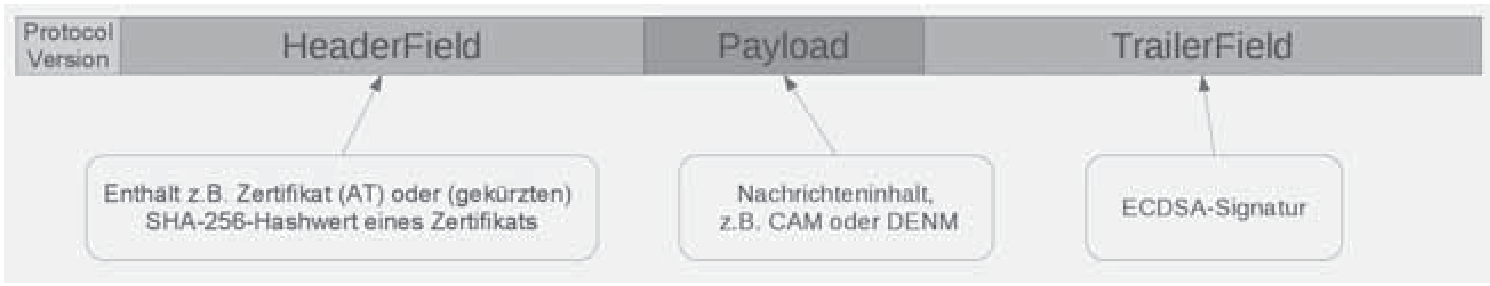
\includegraphics[width=0.7\linewidth]{images/Nachrichtenaufbau}
	\caption[Grobaufbau einer verschlüsselten Nachricht]{Grobaufbau einer verschlüsselten Nachricht \footnotemark}
	\label{fig:nachrichtenaufbau}
\end{figure}
\footnotetext{\emph{Strubbe}, In: DuD 2017, 223}

Im Weiteren wird nur die CAM betrachtet, da die DENM keine personenbezogenen Daten beinhaltet und im datenschutzrechtlichem Sinne kein Problem darstellt \cite{Kiometzis2017}. Der Aufbau einer CAM wird in der Abbildung \ref{fig:cam} dargestellt. Sie besteht aus vier Elementen: Header, CAM Information, Signature und Certificate. Die tatsächliche Information über das Fahrzeug wird im Block CAM Information gespeichert. Er beinhaltet sowohl dynamische Daten (z.B. Last Geographic Position, Speed) als auch statische Daten über das Fahrzeug, die trotz ständigem Pseudonymwechsel identisch bleiben (z.B. Length, Weights). Eine CAM erhält keinen primären Identifikator, aufgrund dessen eine eindeutige Zuordnung zum Fahrzeug möglich wäre.

\begin{figure}
	\centering
	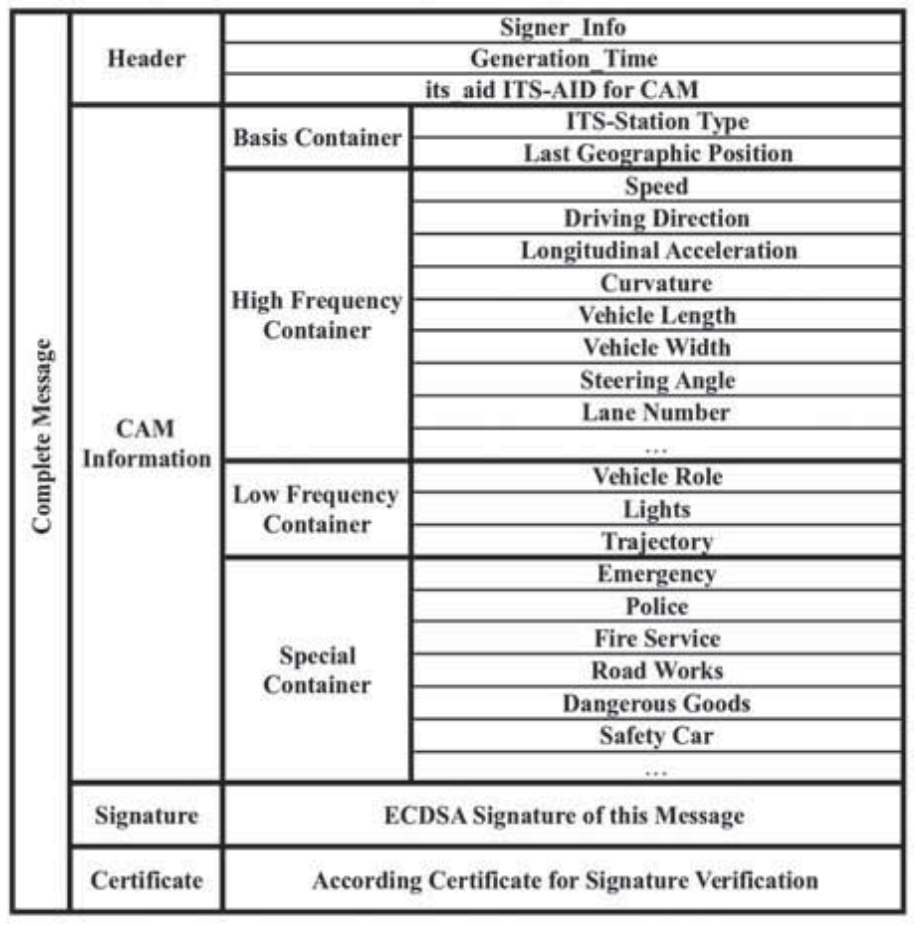
\includegraphics[width=0.4\linewidth]{images/CAM}
	\caption[Detallierter Aufbau einer CAM]{Detallierter Aufbau einer CAM \footnotemark}
	\label{fig:cam}
\end{figure}
\footnotetext{\emph{Kiometzis}, In: DuD 2017, 227}

\section{Anwendbarkeit der DSGVO}
\label{sec:SecondContentSection:SecondSubsection}

Die Datenschutzgrundverordnung (DSGVO) ist eine Verordnung, mit der die Regeln zur Verarbeitung personenbezogener Daten in der Europäischen Union vereinheitlicht werden. Sie ist am 25. Mai 2018 in Kraft getreten und hat zu dem Zeitpunkt geltende Richtlinie 95/46/EG zum Schutz natürlicher Personen bei der Verarbeitung personenbezogener Daten und zum freien Datenverkehr ersetzt. 

In diesem Abschnitt wird diskutiert, ob die Erhebung von Fahrdaten in einer PKI ein datenschutzrechtliches Problem darstellt, und geprüft, ob die DSGVO in diesem Fall anwendbar ist. Des Weiteren werden mögliche Angriffe auf die Pseudonymität der Nachrichten aufgeführt, aufgrund deren Bewegungsprofile von Fahrzeugen erstellt werden können. Aktuell ist die Infrastruktur so konstruiert, dass Fahrzeuge Nachrichten und Zertifikate pseudonym versenden, und keine Zuordnung von mehreren über einen längeren Zeitraum versendeten Nachrichten zu einem Fahrzeug technisch möglich ist. Allerdings gibt es andere Methoden, wodurch solch eine Zuordnung ohne Zustimmung des Fahrers realisiert werden kann, diese werden im Abschnitt \ref{sec:FirstContentSection:ThirdSubSection} beschrieben. Darüber hinaus wird die Anwendbarkeit der DSGVO auf die in CAMs erhaltenen Fahrdaten diskutiert. Falls diese Daten personenbezogen sind, beziehungsweise für eine eindeutige Identifizierung der Person benutzt werden können, fällt ihre Verarbeitung unter DSGVO. Die Datenschutzrechtliche Bedeutung von Bewegungsprofilen wird im Abschnitt \ref{sec:SecondContentSection:SecondSubsection:FirstSubSubsection} diskutiert, und die Möglichkeit zur Herstellung des Personenbezugs wird im Abschnitt \ref{sec:SecondContentSection:SecondSubsection:FirstSubSubsection} analysiert.

\subsection{Datensammlung und -auswertung}
\label{sec:FirstContentSection:ThirdSubSection}

Auch wenn CAMs keine primären Identifikationsmerkmale erhalten, existieren es mehrere Möglichkeiten, um mehere CAMs von einem Fahrzeug miteinander zu verbinden und damit ein Bewegungsprofil von diesem Fahrzeug zu erstellen. Dies kann zu diversen Risiken für die Privatsphäre führen, falls der Personenbezug von diesen Fahrdaten hergestellt werden kann, da der gesamte Fahrweg einer Person offengelegt wird. Im folgenden Abschnitt werden einige Angriffsarten auf die Pseudonymität von CAMs näher beschrieben und analysiert. 

Als erstes Beispiel sei ein sogenannter 'Big Brother Angreifer' angeführt, der eine Infrastruktur von Empfangseinrichtungen in einer geografischen Region betreibt und in der Lage ist, in dieser Gegend CAMs von Fahrzeugen zu erfassen und auszuwerten. Das wäre möglich, indem der Angreifer zum Beispiel eine Fahrzeug-Flotte aufstellt, die eingehende CAMs an einen zentralen Server übermittelt. Auch wenn vorbeifahrende Fahrzeuge ihr Pseudonym jede zehn Sekunden ändern würden, könnten sie mit solch einer Infrastruktur verfolgt werden \cite{Wiedersheim2010}. Da diese Art von Überwachung alle Fahrzeugdaten in der Gegend erfassen würde, könnte sie für breitere Verkehrsanalysen genutzt werden.

Darüber hinaus gibt es einige Möglichkeiten, die Bewegungen von einzelnen Fahrzeugen detailliert aufzuzeichnen. Zum Beispiel kann man mithilfe eines sich mit dem Fahrzeug bewegendes Überwachungstools sogenannte CAM-Traces (Bewegungsprofile) erstellen, d.h. die gefahrene Strecke eines Fahrzeugs und alle von ihm auf dieser Strecke erstellten CAMs. Auch wenn das Fahrzeug regelmäßig seinen Signaturschlüssel wechselt, würde es reichen, nur eine CAM aus der CAM-Trace dem Fahrzeug eindeutig zuzuordnen, um die gesamte CAM-Trace diesem Fahrzeug zuzuordnen \cite{Kiometzis2017}. 

Es existiert eine Reihe von Methoden, um diese Zuordnung technisch durchzuführen. In \cite{Ullmann2016} wurde dargelegt, dass sie aufgrund der sog. Secondary Vehicle Identifier erfolgen kann. Diese wird von diversen drahtlosen Schnittstellen im Auto zur Verfügung gestellt (z.B. eine Headunit, die eine öffentliche Bluetooth-Schnittstelle mit einem nutzerfreundlichen Namen besitzt). Die Secondary Vehicle Identifiers sind einfach zu erfassen und können einer eindeutigen Zuordnung der empfangenen CAM-Trace zum Fahrzeug dienen. 

\subsection{Bewegungsprofile und Verhaltensprofile}
\label{sec:SecondContentSection:SecondSubsection:FirstSubSubsection}

Wie vorhin erwähnt, erhalten CAMs keine primären Identifikationsmerkmale, jedoch ist es möglich, mithilfe von einer geeigneten Infrastruktur Bewegungsprofile von Fahrzeugen zu erstellen. Außerdem enthalten CAMs statische Attribute wie zum Beispiel die Fahrzeuglänge und dessen Gewicht, die eine zusätzliche Kennzeichnung von einem Fahrzeug erlauben. So wäre es unter Umständen möglich, ein bestimmtes Modell von einem bestimmten Hersteller nur aus der CAM zu erkennen. In wenig befahrenen Gebieten kann dies zu einer eindeutigen Identifizierung von dem Fahrzeug und einer Zuordnung zum ganzen CAM-Trace führen. Darüber hinaus kann man mithilfe von Secondary Vehicle Identifiers (z.B. einer öffentlich verfügbaren Bluetooth-Schnittstelle) diese Zuordnung durchführen. Letztens, da die CAM-Daten mit einer hohen Frequenz versendet werden, kann der Fahrweg mit einer hohen Zuverlässigkeit voraus- und zurückberechnet werden. 

Somit ist es grundsätzlich möglich, aus einem flächendeckenden Datenbestand aus CAMs über einen längeren Zeitraum Bewegungsprofile zu erstellen, und somit gegebenenfalls auch Verhaltensprofile. In \cite{Dettki2005} wurde zum Beispiel nachgewiesen, dass anhand der Lenkbewegungen ruhige von nervösen Fahrer unterschieden werden können. Außerdem wäre es durch die Anwendung von künstlicher Intelligenz und maschinellem Lernen durchaus möglich, große Datenbestände von Bewegungsprofilen und somit die zugehörigen Fahrer zu klassifizieren, falls Personenbezug hergestellt werden kann. 

% Hier noch mehr über verschiedene Probleme schreiben

\subsection{Herstellbarkeit Personenbezug}
\label{sec:SecondContentSection:SecondSubsection:SecondSubSubsection}

Nach Art. 4 Nr. 1 DSGVO sind personenbezogene Daten alle Informationen, die sich auf eine identifizierte oder identifizierbare natürliche Person beziehen. Selbst wenn CAMs direkt keine primären Identifikationsmerkmale enthalten (z.B. die Fahrzeugidentifizierungsnummer), kann deren Personenbezug grundsätzlich mit Zusatzwissen hergestellt werden. Technisch kann das durch eine Auflösung des Pseudonyms bei einer Certification Authority erfolgen \cite{Kiometzis2017}, aber auch durch andere Wege. Zum Beispiel kann man anhand einer CAM-Trace aufgrund der am meisten gefahrenen Strecken den Wohn- und Arbeitsort einer Person identifizieren. Außerdem wäre es zum Beispiel möglich, durch Datenanalyse die Outliers in der Menge von den aufgezeichneten CAM-Traces identifizieren und versuchen, sie auf Personen mit entsprechendem Tagesablauf zurückzuführen. Besonders in wenig befahrenen Gebieten wäre diese Technik erfolgreich. Letztendlich wäre in vielen Situationen der einfachste Weg, vor Ort das Fahrzeug zu identifizieren (z.B. durch aufgezeichnete Videos oder Zeugenaussagen), und später aus dem Datenbestand die entsprechende CAM-Trace auszusuchen. Alle oben ausgeführten Techniken voraussetzen natürlich eine umfassende Erfassung von Fahrdaten und einen vorhandenen Bestand von Bewegungsprofilen (z.B. den in Kapitel \ref{sec:FirstContentSection:ThirdSubSection} beschriebenen Big Brother Angreifer).

Eine besondere Sensibilität allein aus der Art der Daten einer CAM wird nach Art. 9 EU-DSGVO nicht begründet \cite{Weichert2016}. Allerdings genügt für die datenschutzrechtliche Betrachtung bereits die abstrakte rechtliche Möglichkeit der Informationsverknüpfung. Das heißt: falls es technisch möglich ist, den Fahrzeughalter aus den Daten zu identifizieren, fällt die Erhebung von CAMs unter die DSGVO - unabhängig davon, ob die Voraussetzungen dafür tatsächlich erfüllt sind  \footnote{\emph{Specht/Mantz}, Handbuch Europäisches und deutsches Datenschutzrecht, 1. Aufl., 2019, Rn. 12, 13}. Dies könnte sich zukünftig mit der Einsetzung von Shared Mobility-Konzepten ändern, falls man überwiegend nur kurzzeitig ein Fahrzeug anmietet und die Fahrzeugnummer nicht mehr auf natürliche Personen zurückgeführt werden kann. 


\section{Vereinbarkeit mit datenschutzrechtlichen Prinzipien}
\label{ch:SecondContentSection}

Da die DSGVO auf die in CAMs enthaltenen Daten anwendbar ist, muss sie während der Bearbeitung und ggf. Speicherung der Fahrdaten stets eingehalten werden. Dies ist von großer Wichtigkeit für Betreiber der PKI, Autohersteller und andere an C-ITS beteiligten Unternehmen, da die Nichteinhaltung der DSGVO für sie mit hohen Geldstrafen drohen könnte. In diesem Kapitel werden relevante Grundsätze der DSGVO angefürt und deren Einhaltung geprüft. Für jeden Grundsatz werden die Datenschutzmaßnahmen und offene Fragen beschrieben, die bei der Einführung einer C-ITS beachtet werden müssen. 

\subsection{Grundsatz der Datenminimierung}

Nach Art.5 Abs.1c DSGVO ist der Grundsatz der Datenminimierung folgendermaßen definiert: "Personenbezogene Daten müssen dem Zweck angemessen und erheblich sowie auf das für die Zwecke der Verarbeitung notwendige Maß beschränkt sein". Im Kontext von Intelligenten Verkehrssystemen heißt es, dass eine Erstellung von Bewegungs- und Verhaltensprofilen verhindert werden muss. Nach \cite{Kiometzis2017} ergeben sich demzufolge 3 Maßnahmen, die für Datenminimierung in C2C sorgen könnten:
\begin{itemize}
	\item Transparenzgrundsatz: dem Fahrzeugführer soll transparent angezeigt werden, dass sich das Fahrzeug am Versand von CAMs und DENMs beteiligt. 
	\item C-2-C Deaktivierungsmöglichkeit: der Fahrzeugführer muss selektiv in der Lage sein, den aktiven Versand von CAMs und DENMs zu deaktivieren.
	\item Vorkonfigurierte C-2-C Standardeinstellung: als Standardkonfiguration wäre es ausreichend, wenn Fahrzeuge CAMs und DENMs empfangen können aber ausschließlich DENMs verschicken
\end{itemize}

Außerdem sollte man beim Entwurf einer C-ITS darauf achten, dass eine geeignete Pseudonimisierung erfolgen kann. Die grundlegende Anforderung ist hier, dass die Verschlüsselungs-Zertifikate sich regelmäßig ändern müssen, so dass man die CAMs bei der zentralen Sammelstelle nicht auf die gleiche Person zurückführen kann. Wir haben aber bereits gesehen, dass die Zuordnung zur Identität einigermaßen auch mit sich ständig wechselnden Zertifikaten erfolgen kann. Daher stellt sich die Frage, welche Daten in CAMs gespeichert werden müssen, und ob ein Nachrichtenformat für alle Zwecke ausreichend ist.

Aktuell sind CAMs für fast alle Verkehrsszenarien vorgesehen, was aus Sicht der Datenschutz nicht optimal ist. Generell sind aber viele Daten darin für die meisten Anwendungen unnötig, was dem Grundsatz der Datenminimierung widerspricht. Daher wird es in \cite{Kiometzis2017} vorgeschlagen, für die häufigsten Anwendungsszenarien einen minimalen Nachrichtentyp zu nutzen, der nur die erforderlichen Daten erhält. Wenn wir uns aber bei Day 3 befinden und echte kooperativen Szenarien in Frage kommen, sollte dafür ein zusätzlicher verbindungsorientierter Kommunikationsstandard genutzt werden. So kann man die Daten auf eine geeignete Weise voneinander trennen ohne Verlust der Funktionalität, und somit einen datenschutzrechtlichen Kompromiss erreichen.

\subsection{Grundsatz der Integrität und Vertraulichkeit}

Der Grundsatz der Integrität und Vertraulichkeit (Art.5 Abs.1c DSGVO) sieht vor, dass "personenbezogene Daten in einer Weise verarbeitet werden, die eine angemessene Sicherheit der personenbezogenen Daten gewährleistet, einschließlich Schutz vor unbefugter oder unrechtmäßiger Verarbeitung und vor unbeabsichtigtem Verlust, unbeabsichtigter Zerstörung oder unbeabsichtigter Schädigung durch geeignete technische und organisatorische Maßnahmen". Dies entspricht den Vorgaben des Art. 10 IVS-RL, nach dem die Mitgliedstaaten sicherstellen sollten, dass personenbezogene Daten gegen Missbrauch, d.h. insbesondere unrechtmäßigen Zugriff, Veränderung oder Verlust, geschützt werden. Weiterhin sollen für den Betrieb von C-ITS-Anwendungen und -Diensten soweit wie möglich anonymisierte Daten verwendet werden, um mögliche Schaden zu verringern\footnote{\emph{Jochum}, In: ZD 2020, 497}. 

Entscheidend ist hier die Anforderung an die Flüchtigkeit der CAMs. Es muss eine Technik für C-ITS entwickelt werden, die eine unbefugte Nutzung der in CAMs enthaltenden Daten unterbinden kann \cite{Kiometzis2017}, oder nach einer kurzen Zeit den Inhalt davon invalidiert. Das Prinzip davon wäre analog zu anderen Diensten, wo die Verbreitung der Inhalten kontrolliert wird, z.B. Musikanwendungen, die das Abspielen von Dateien nur nach dem Kauf erlauben. 

Darüber hinaus besteht nach Art.33 DSGVO unter Umständen eine Pflicht, Verletzungen des Schutzes personenbezogener Daten an die Aufsichtsbehörde zu melden. Art.35 DSGVO sieht außerdem vor, dass im Falle von einem hohen Risiko für die Rechte und Freiheiten natürlicher Personen, das durch die Verwendung einer neuen Technologie entsteht, eine Abschätzung der Folgen für den Schutz personenbezogener Daten durchgeführt werden kann. Das ist besonders relevant im Kontext von C-ITS, da mithilfe der neuen AI-Technologien Einsicht in pseudonyme Fahrdaten genommen werden kann, wodurch möglicherweise Personenbezug entstehen könnte\footnote{\emph{Seewald}, In: RAW 2020, 130}. 

\subsection{Grundsatz der Zweckbindung}

Nach Art.5 Abs.1b DSGVO gilt der Grundsatz der Zweckbindung, nach dem personenbezogenen Daten nur für festgelegte, eindeutige und legitime Zwecke verarbeitet werden müssen. Das heißt: falls personenbezogene Daten erhoben werden, muss der Grund dafür klar definiert und eingehalten werden, durch eine Einwilligung oder auf eine andere Weise (Art.6 Abs.1a DSGVO). Als Ausnahme gelten Archivzwecke, wissenschaftliche oder historische Forschungszwecke und statistische Zwecke - sie gelten nach Art.89 Abs.1 nicht als unvereinbar mit den ursprünglichen Zwecken. 

Im Kontext von C-ITS heißt es, dass die Zweitnutzung der Fahrdaten nur aufgrund einer Zustimmung erfolgen werden darf. Die Standortdaten allein unterliegen im allgemeinen Datenschutzrecht keinem besonderen Schutz; falls es jedoch möglich ist, Bewegungsprofile aus solchen Daten zu generieren, muss ebenfalls die Zweitnutzung der Daten gesetzlich geregelt werden. Das heißt, jegliche Datenverarbeitung über die ursprüngliche Zwecke hinaus (individualisierte Zweitnutzung) muss explizit eine Einwilligung voraussetzen\footnote{\emph{Weichert}, In: SVR 2016, 361}.

Außerdem ist es bei vielen C2X Anwendungen der Fall, dass auch andere Daten zusätzlich zu den Standortdaten regelmäßig versendet werden. Aus dieser Information können mehrere Datenspuren nicht nur zum Aufenthalt des Fahrzeughalters entstehen, was eine Dauerüberwachung verursachen kann\footnote{\emph{Weichert}, In: SVR 2014, 241 f.}. Das ist ein weiterer Grund dafür, die Zweitnutzung jeglicher Fahrdaten nur über eine explizite Einwilligung zu erlauben. 

Neben der individualisierten Zweitnutzung von Fahrdaten gibt es andere Möglichkeiten, für die der Grundsatz der Zweckbindung entfallen kann. Im Falle von kollektiver Datennutzung findet die Anonymisierung der Daten vor der Zweckänderung statt, was eine Zweitnutzung ohne Zustimmung von jedem einzelnen Verkehrsteilnehmer erlaubt. Dies setzt aber einen großen Datenbestand voraus, in dem auf keine einzelne Person zurückgeführt werden kann, und aus dem keine Bewegungsprofile generiert werden können. Für anonymisierte Fahrdaten ergeben sich ebenfalls mehrere Nutzungsfälle, z.B. Verkehrslenkung, Gefahrenabwehr, Verkehrsstatistik oder -forschung\footnote{\emph{Weichert}, In: SVR 2016, 367}.

\subsection{Recht auf Datenübertragbarkeit}

Neben den Grundsätzen aus Art.5 Abs.1 DSGVO muss auch der Art.20 DSGVO erwähnt werden, wodurch das Recht auf Datenübertragbarkeit vorgeschrieben wird. Nach dem Artikel hat die betroffene Person das Recht, "die sie betreffenden personenbezogenen Daten, die sie einem Verantwortlichen bereitgestellt hat, in einem strukturierten, gängigen und maschinenlesbaren Format zu erhalten". Außerdem ist dem Betroffenen das Recht eingeräumt, seine Daten von einem Anbieter zu einem anderen zu übertragen. Dies entspricht dem Recht auf informationelle Selbstbestimmung nach Art.8 GRCh und ermöglicht es, die Daten ohne Behinderung verschiedenen Interessierten zur Verfügung zu stellen, z.B. Autoherstellern, Vertragshändlern, Versicherungen und Leasinggebern\footnote{\emph{Klink-Straub/Straub}, In: ZD 2018, 459}.

Hier ist es wichtig zu betonen, dass der Artikel sich auf die Fahrdaten bezieht, die vom Betroffenen bereitgestellt wurden. Diese Bedingung wird erfüllt, wenn die Daten wissentlich und aktiv von betroffenen Personen mitgeteilt wurden\footnote{\emph{Art. 29-Datenschutzgruppe}, Leitlinien zum Recht auf Datenübertragbarkeit, S. 11}, aber auch wenn die Daten durch die Nutzung des Dienstes von der Person aufgezeichnet wurden\footnote{\emph{Strubel}, In: ZD 2017, 355, 357}. Im Gegensatz dazu sind die Daten, die durch eine Auswertung der Fahrdaten entstanden sind, keine vom Fahrer bereitgestellte Daten\footnote{\emph{Art. 29-Datenschutzgruppe}, (o. Fußn. 22)}. Zum Beispiel sind die Rückschlüsse auf das Fahrverhalten aus den gesammelten Daten ("Person A ist ein vorsichtiger Fahrer") keine bereitgestellten Daten. 

Die wichtigste Herausforderung im Kontext von C-ITS besteht zunächst darin, die beim Fahrzeughersteller oder beim Betreiber der PKI gespeicherten Daten im maschinenlesbaren Format betroffenen Personen zugänglich zu machen. Um Art.20 Abs.4 DSGVO gerecht zu werden, müssen die Verantwortlichen dabei die Rechte der Drittbetroffenen beachten, da beim Bereitstellen der Daten möglicherweise die Daten der anderen Verkehrsteilnehmern übermittelt werden könnten\footnote{\emph{Klink-Straub/Straub}, In: ZD 2018, 463}. Letztens müssen die Datenschutzmechanismen bei den Empfängern der Daten (z.B. Händler, Werkstätten, Versicherungen) unter die Lupe genommen werden, da sie beim Empfang der Daten nach Art.20 Abs.2 DSGVO selbst zu Verantwortlichen werden.



%Add additional content sections if required by adding new .tex files in the
%\code{sections/} directory and adding an appropriate 
%\code{\textbackslash input} statement in \code{thesis.tex}. 
%%% ---------------------
%% | / Example content |
%% ---------------------